% MuleGuard AI --- CyberShield prototype submission
% Generated by src/make_paper_tex.py from reports/*.json. Do not hand-edit
% numbers here; re-run the pipeline and regenerate instead.
\documentclass{article}
\usepackage{spconf,amsmath,graphicx,hyperref,booktabs}

% spconf leaves no gap below a caption, so a table caption sitting above its
% tabular collides with the top rule. Give it a little air.
\setlength{\abovecaptionskip}{6pt}
\setlength{\belowcaptionskip}{4pt}

\title{MULEGUARD AI: LEAKAGE-HARDENED MONEY-MULE DETECTION AND A DATASET INTEGRITY AUDIT}

\name{1st Given Name Surname, 2nd Given Name Surname, 3rd Given Name Surname}
\address{Department Name\\
	Institution Name\\
	City, Country}

\begin{document}
\ninept
\maketitle

\begin{abstract}
Money-mule accounts settle digital payment fraud but are vanishingly rare in
labelled banking data. We present MuleGuard AI, a detection pipeline for
9,082 accounts containing 81 confirmed mules
(0.8919\%). Our primary finding is that the benchmark itself is
contaminated: positives and negatives are drawn from disjoint monthly extracts,
and a model given only the pattern of blank cells---every value discarded---reaches
AUPRC 0.824 against a 0.0089 random baseline. We supply
falsification tests that make this measurable. We further contribute a leakage
taxonomy that classifies fields by meaning rather than correlation, catching an
outcome flag correlated just 0.05 with the target, and 29 named
mule-typology features. Under nested repeated cross-validation, in which
selection, calibration and the operating threshold are all fitted in-fold, the
ensemble reaches precision $0.976 \pm 0.067$ at recall $0.692 \pm 0.129$. We
argue these are an upper bound on what this dataset can establish.
\end{abstract}

\begin{keywords}
Money-mule detection, anti-money laundering, class imbalance, target leakage,
dataset integrity
\end{keywords}

\section{Introduction}
\label{sec:intro}

A money mule is a bank account, opened by a real customer who is coerced,
recruited or paid, that receives criminal proceeds and forwards them onward
within hours. Mules sit between the fraud victim and the organiser, and freezing
one strands funds that are otherwise irrecoverable. India's real-time payment
rails make this faster and more damaging, and the Reserve Bank of India requires
that automated action against a customer account be explainable
\cite{rbi2016kyc}.

Three difficulties compound. Mules are extremely rare, so accuracy is
meaningless---predicting that every account is normal scores 99.11\% here---and
the precision-recall curve is the appropriate summary \cite{davis2006pr}. Mules
are behaviourally camouflaged: the account belongs to a genuine customer with a
genuine history, so unsupervised anomaly detection has little purchase, which our
ablation confirms sharply. Finally, labels in this domain are the output of an
investigation, and that process leaves traces a model will exploit
\cite{kaufman2012leakage}.

This last point dominates. While building the detector we found the supplied
benchmark cannot support an honest performance estimate, and that the
contamination is invisible to standard defences. We therefore present the
integrity audit as our primary contribution, with the detector as the vehicle
that exposed it.

\section{Dataset and integrity audit}
\label{sec:data}

The dataset comprises 9,082 accounts and
3,924 anonymised features, with a separate dictionary
mapping each to a named banking variable. Features follow a regular grammar: a
statistic (ratio, deviation, average, extremum) over a payment channel (cash,
cheque, UPI, ATM, online transfer, Aadhaar Payment Bridge) in a direction
(credit, debit) over a window (7, 14, 31 days). A tail block holds demographics,
alert counts by time of day, and investigation metadata.

\subsection{Leakage a correlation threshold cannot see}

Four fields record an alert's resolution status and two record how long the
investigation took. All six exist only after an analyst closes a case, so none is
available when an account must actually be scored. Their correlations with the
target span two orders of magnitude: {\tt FRAUD\_SUSPECTED} at 0.969 is caught
by any threshold, while {\tt FALSE\_POSITIVE} at 0.055 is caught by none---yet
it encodes the same verdict, merely inverted. We therefore classify leakage by
what a field \emph{means}, using the dictionary, and treat correlation only as a
backstop.

\subsection{A structural confound}

Table~\ref{tab:months} gives the complete cross-tabulation of class against
extract month. Every negative is drawn from the October extract and every
positive from September, November and December. No month contains both classes,
so the month column alone separates them---and it is not a property of any
customer, but a record of which extraction run produced the row.

\begin{table}[htb]
\centering
\caption{Class composition by monthly extract. No month contains both classes.}
\label{tab:months}
\vspace{1ex}
\begin{tabular}{lrr}
\toprule
Extract month & Normal & Mule \\
\midrule
Dec25 & 0 & 10 \\
Nov25 & 0 & 23 \\
Oct25 & 9,001 & 0 \\
Sep25 & 0 & 48 \\
\bottomrule
\end{tabular}
\end{table}

Dropping the month column does not help. Because the classes occupy disjoint
extracts, any characteristic that varies between extraction runs aligns perfectly
with the label while describing nothing about behaviour. Adversarial validation
cannot diagnose this, since a classifier trained to predict the extract is by
construction the classifier that predicts the label.

\subsection{Falsification tests}

We constructed three tests, each supplying a model with information that cannot
identify a mule. All should score near the 0.0089 baseline if the data is
sound. In test A every value is discarded and the model sees only whether each
cell was populated---a property of the extraction job, not the customer. In test
B the model receives 250 columns drawn from the 3,174 whose
individual correlation is below 0.05, none of which can identify a mule alone. In
test C the labels are permuted.

Table~\ref{tab:falsify} reports the outcome. Test C collapsing to the baseline
confirms the harness is sound, so the first two results are genuine properties of
the data rather than a defect in our code. The conclusion is unavoidable: any
figure computed on this dataset, by any team and any method, measures extract
provenance in addition to mule behaviour, and the two cannot be separated within
this file. Section~\ref{sec:results} should be read with that attached.

\begin{table}[htb]
\centering
\caption{Falsification tests. Information that cannot identify a mule still
separates the classes.}
\label{tab:falsify}
\vspace{1ex}
\begin{tabular}{clrr}
\toprule
Test & Information supplied & AUPRC & AUROC \\
\midrule
A & Blank/not-blank only & 0.824 & 0.993 \\
B & 250 cols, $|r| < 0.05$ & 0.736 & 0.973 \\
C & As B, labels shuffled & 0.0094 & 0.528 \\
\midrule
--- & Random guess & 0.0089 & 0.500 \\
\bottomrule
\end{tabular}
\end{table}

\section{Method}
\label{sec:method}

Fig.~\ref{fig:arch} shows the pipeline. We highlight only what a reader needs
to trust the numbers.

\begin{figure*}[htb]
\centering
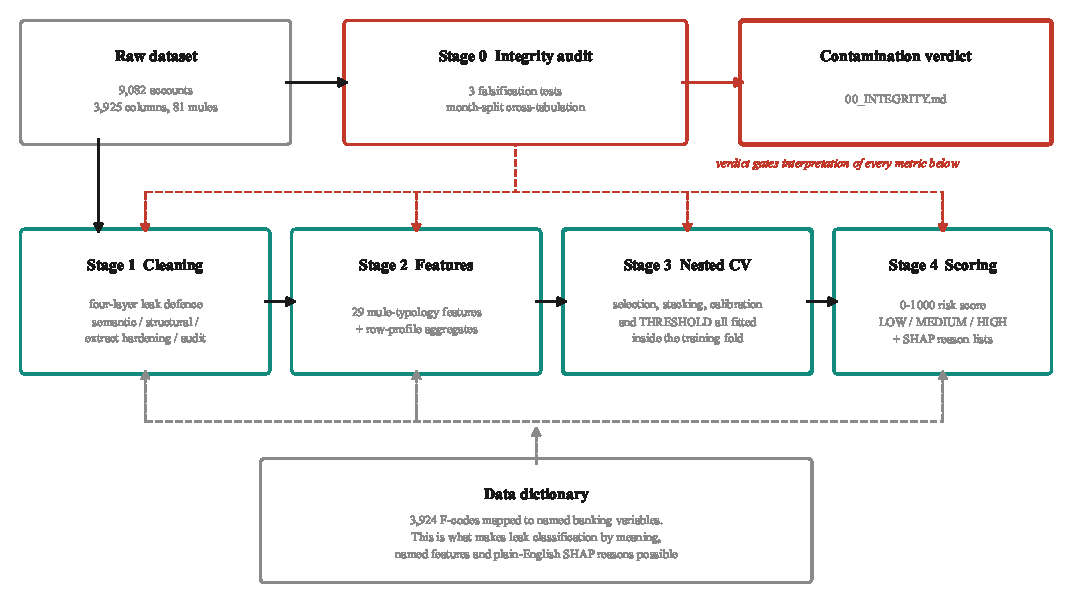
\includegraphics[width=\textwidth]{figures/fig1_architecture}
\caption{MuleGuard AI pipeline. Stage 0 runs before any modelling and its
verdict qualifies every metric produced downstream (red). Leak defences
concentrate in Stage 1. In Stage 3 every component that touches the label ---
feature selection, stacking weights, the calibration map and the decision
threshold --- is fitted inside the training fold and applied frozen to
validation rows. The data dictionary is drawn as a bus because it is
cross-cutting rather than a pipeline step: it supplies the named semantics that
Stages 1, 2 and 4 depend on. The graph stage is omitted from the figure; it
detects the absence of counterparty identifiers and disables itself.}
\label{fig:arch}
\end{figure*}

\textbf{Preserving destroyed information.} Eight columns are categorical,
including occupation, gender and product. Coercing the matrix to numeric---the
customary step---converts them to missing values that are then dropped as sparse.
This discards real signal: mule rates by occupation range from 0.45\% for
homemakers to 1.94\% for students against a 0.89\% base. We encode the account-age
bucket ordinally and the rest as indicators. We also revisit imputation: for
absolute activity aggregates a missing value means the activity never occurred,
so we zero-fill 78,919 values across
1,357 columns rather than inventing activity
through median imputation.

\textbf{Four-layer leakage defence.} Layer one removes post-outcome fields
semantically. Layer two removes structural artefacts of sample assembly.
Layer three, \emph{extract hardening}, removes any column whose blank rate differs
between classes by more than ten percentage points, on the grounds that cell
population is decided by the extraction job; this dropped
574 columns. It uses the label, but only
ever removes columns, so it can make the reported result worse and never better.
Layer four is a separation audit scanning every surviving column for disjoint
class ranges, which reports clean after the first three.

\textbf{Mule-typology features.} A mule receives funds and forwards them almost
immediately, retains little, operates in bursts, favours digital rails, and
belongs to a customer whose profile does not match the volume. We encode each
clause as a named family---pass-through ratio, turnover over balance, burst,
cash-out share, channel concentration, ticket size, night-alert share, balance
volatility, occupation divergence---29 features in total.

\textbf{Nested validation.} The ensemble stacks an isolation forest
\cite{liu2008isolation}, XGBoost \cite{chen2016xgboost} and LightGBM
\cite{ke2017lightgbm} through a logistic meta-learner \cite{wolpert1992stacking}
with isotonic calibration \cite{zadrozny2002calibration}. Missing values are
imputed with medians learned inside the training fold rather than across the
whole matrix, which removes a transductive leak and is also the only defensible
treatment for a single account scored at run time. Every component
touching the label---selection, base models, stacking weights, the calibration
map, \emph{and the decision threshold}---is fitted inside the training fold and
applied frozen to unseen validation rows. This matters: calibrating on pooled
out-of-fold predictions and scoring those same values inflates the result, and
selecting the threshold that maximises precision on a curve then reporting that
precision is optimistic by construction \cite{cawley2010overfitting}. We prefer
instance reweighting to synthetic oversampling \cite{chawla2002smote}, which with
65 training positives across hundreds of dimensions fabricates regions of feature
space for which no evidence exists. Because a single split places about 16 mules
per fold, we repeat the procedure across shuffles and report mean $\pm$ standard
deviation.

\section{Results}
\label{sec:results}

Table~\ref{tab:results} reports the calibrated ensemble. At the precision-first
operating point it attains precision $0.976 \pm 0.067$ at recall
$0.692 \pm 0.129$, with AUPRC $0.854 \pm 0.076$ against a
0.0089 baseline; summed across folds,
168 true positives against 6 false positives. A
second operating point trades precision to $0.531 \pm 0.145$ for recall
$0.880 \pm 0.099$, appropriate when a reviewed alert costs minutes and a missed
mule costs a laundering channel.

\begin{table}[htb]
\centering
\caption{Detection performance and per-model ablation, nested repeated
cross-validation (mean $\pm$ std across folds).}
\label{tab:results}
\vspace{1ex}
\begin{tabular}{lrr}
\toprule
Metric & Precision-first & High-recall \\
\midrule
Precision & $0.976 \pm 0.067$ & $0.531 \pm 0.145$ \\
Recall & $0.692 \pm 0.129$ & $0.880 \pm 0.099$ \\
F1 & $0.800 \pm 0.088$ & $0.647 \pm 0.095$ \\
\midrule
\multicolumn{3}{l}{\emph{Per-model AUPRC (threshold-independent)}} \\
Isolation forest & \multicolumn{2}{r}{$0.007 \pm 0.001$} \\
LightGBM & \multicolumn{2}{r}{$0.818 \pm 0.080$} \\
XGBoost & \multicolumn{2}{r}{$0.894 \pm 0.061$} \\
Calibrated ensemble & \multicolumn{2}{r}{$0.854 \pm 0.076$} \\
\bottomrule
\end{tabular}
\end{table}

The isolation forest result is the informative one. At AUPRC $0.007 \pm 0.001$ and
AUROC 0.314 it performs \emph{worse than random}. This
is not a defect but a finding, consistent with the criminology: a mule account
belongs to a real customer with an ordinary history, and is valuable to the
organiser precisely because it does not look anomalous. Unsupervised outlier
detection is the wrong tool here, and proposals leading with it deserve
suspicion.

Fig.~\ref{fig:shap} ranks features by mean absolute SHAP contribution
\cite{lundberg2017shap}, computed per fold on validation rows only, so each
account is explained by the same out-of-fold model that scored it rather than by
a final model refit on every row including that account.
6 of the top 12 are engineered in this work
rather than supplied columns, indicating the typology encoding contributes
materially rather than restating what the raw matrix already exposed. Among
supplied columns, deviations of non-cash non-cheque volume from the occupation
cohort dominate---the profile-mismatch signal appearing directly.

\begin{figure}[htb]
\centering
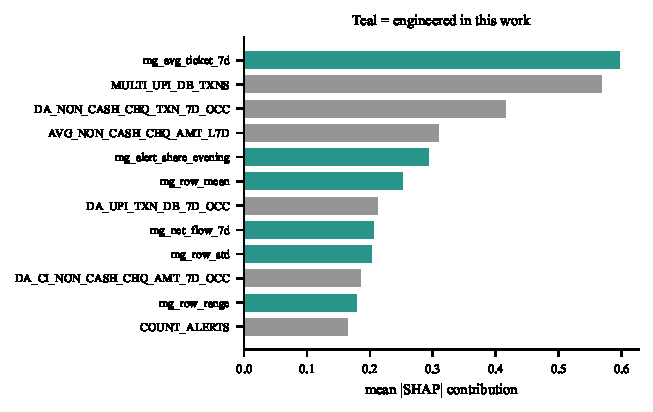
\includegraphics[width=\columnwidth]{figures/fig3_shap}
\caption{Top features by mean absolute SHAP value. Features engineered in this
work are shown in teal, supplied dictionary variables in grey.}
\label{fig:shap}
\end{figure}

The 0--1000 band edges are not chosen by hand. The high-risk edge is the
operating threshold that held precision $\geq$ 0.9 on inner
folds, and the medium edge is the analyst-review-queue threshold; both are
averaged over folds and both were fixed before any validation row was seen. A
band boundary therefore reports a fitted decision rather than a round number.

Operationally, the high-risk band holds 53 accounts of which
53 are confirmed mules (band precision
1.00), capturing 65\% of all
mules in a queue that is 0.58\% of the
portfolio. Reviewing well under one percent of accounts surfaces two thirds of
the mule population.

\section{Discussion and conclusion}
\label{sec:discussion}

The results above are strong, and we do not believe they measure mule detection
capability. Section~\ref{sec:data} establishes that an uninformative view of the
same data achieves comparable separation, so a substantial and unquantifiable
share reflects the extract a row came from. Our hardening removes the artefact
where it is identifiable; it cannot remove what is not. A behavioural feature
that also drifts between months is confounded, and no modelling choice separates
the two within this file. The remedy is a sampling change, not a modelling one:
negatives drawn from the same months as positives would let month be conditioned
on. This affects every team working from this release.

Further limitations bear statement. The dataset is an account-level matrix with
no counterparty identifiers, so the graph component detects their absence and
disables itself rather than fabricating an edge list; network-propagation claims
cannot be evaluated here. Hyperparameters remain at conservative defaults, since
tuning against a confounded objective optimises the artefact. And
81 positives is a small sample---the standard deviations reported are
wide enough that differences of a few points should not be considered
meaningful.

We suggest the falsification protocol of Section~\ref{sec:data} deserves wider
use. It is inexpensive, requires no knowledge of the modelling approach, and here
was the difference between reporting a headline result and understanding what
that result measured \cite{hackathon2026}.

\section{Acknowledgment}

The authors thank the organisers, Bank of India and the Indian Institute of
Technology Hyderabad, for the dataset and the accompanying data dictionary. The
dictionary proved essential rather than incidental: without documented variable
semantics neither the meaning-based leakage taxonomy nor the named feature
families could have been constructed. The integrity findings are offered in a
collaborative spirit---an observation intended to strengthen the benchmark for
all participants and for future releases, not a criticism of those who assembled
and shared it.

\bibliographystyle{IEEEbib}
\bibliography{refs}

\end{document}
